\section{DNS dataset and preprocessing}

The reference data used in this work are generated by Direct Numerical
Simulations of the Rayleigh--Taylor instability. This choice is motivated by
the need for high-fidelity fields: lower-fidelity turbulence models may be
useful in other contexts, but they introduce closure assumptions that are not
desirable here because the objective is precisely to learn the distribution of
physically resolved density fields.

The simulations are produced with a pseudo-spectral solver on two-dimensional
periodic domains initialized with perturbed density interfaces. Each stored
sample corresponds to a snapshot of the temporal evolution of the instability.
The resulting fields contain both large coherent structures and fine
interfacial fluctuations, which makes them relevant for both direct and
multi-resolution generative modeling.

Although DNS provide high-fidelity information, their computational cost
remains substantial because all dynamically relevant scales must be resolved.
As a consequence, the available dataset is relatively small: it is built from
roughly 60 independent simulations and, after preprocessing and filtering,
contains fewer than 7000 images split into training, validation, and test
subsets. This limited size is an important methodological constraint because it
increases the risk of overfitting and reduces the diversity available to the
generative models.

\subsection{Geometric constraints and cropping}

Unlike generic computer vision datasets, the geometry of the raw RTI fields is
not arbitrary. The horizontal direction is periodic, so the domain width must
remain large enough to prevent the largest coherent structures from interacting
too strongly with their periodic images. If $L_x$ denotes the horizontal
domain size and $L_b$ the diameter of the largest bubbles, one seeks to remain
in a regime such that

\begin{equation}
    L_b \ll L_x,
\end{equation}

or more conservatively

\begin{equation}
    L_b \lesssim \frac{L_x}{4}.
\end{equation}

The vertical direction follows a different constraint because the mixing layer
grows under gravity and therefore requires a longer observation window. The raw
simulations are consequently produced on domains of size $128\times512$.

Since the baseline model is trained on square inputs, the original fields are
cropped to a square field of view. This cropping is retained only when the full
mixing zone remains inside the selected window. Let $y_b(t)$ and $y_s(t)$
denote the lowest bubble tip and the highest spike tip. The retained crop must
satisfy

\[
y_{\min}^{\mathrm{crop}} < y_b(t)
\quad\text{and}\quad
y_s(t) < y_{\max}^{\mathrm{crop}},
\]

so that the full physically relevant interface dynamics remains visible.
The retained observation window and the associated mixing-zone constraint are
shown in Figure~\ref{fig:zone_melange}.

\begin{figure}[H]
\centering
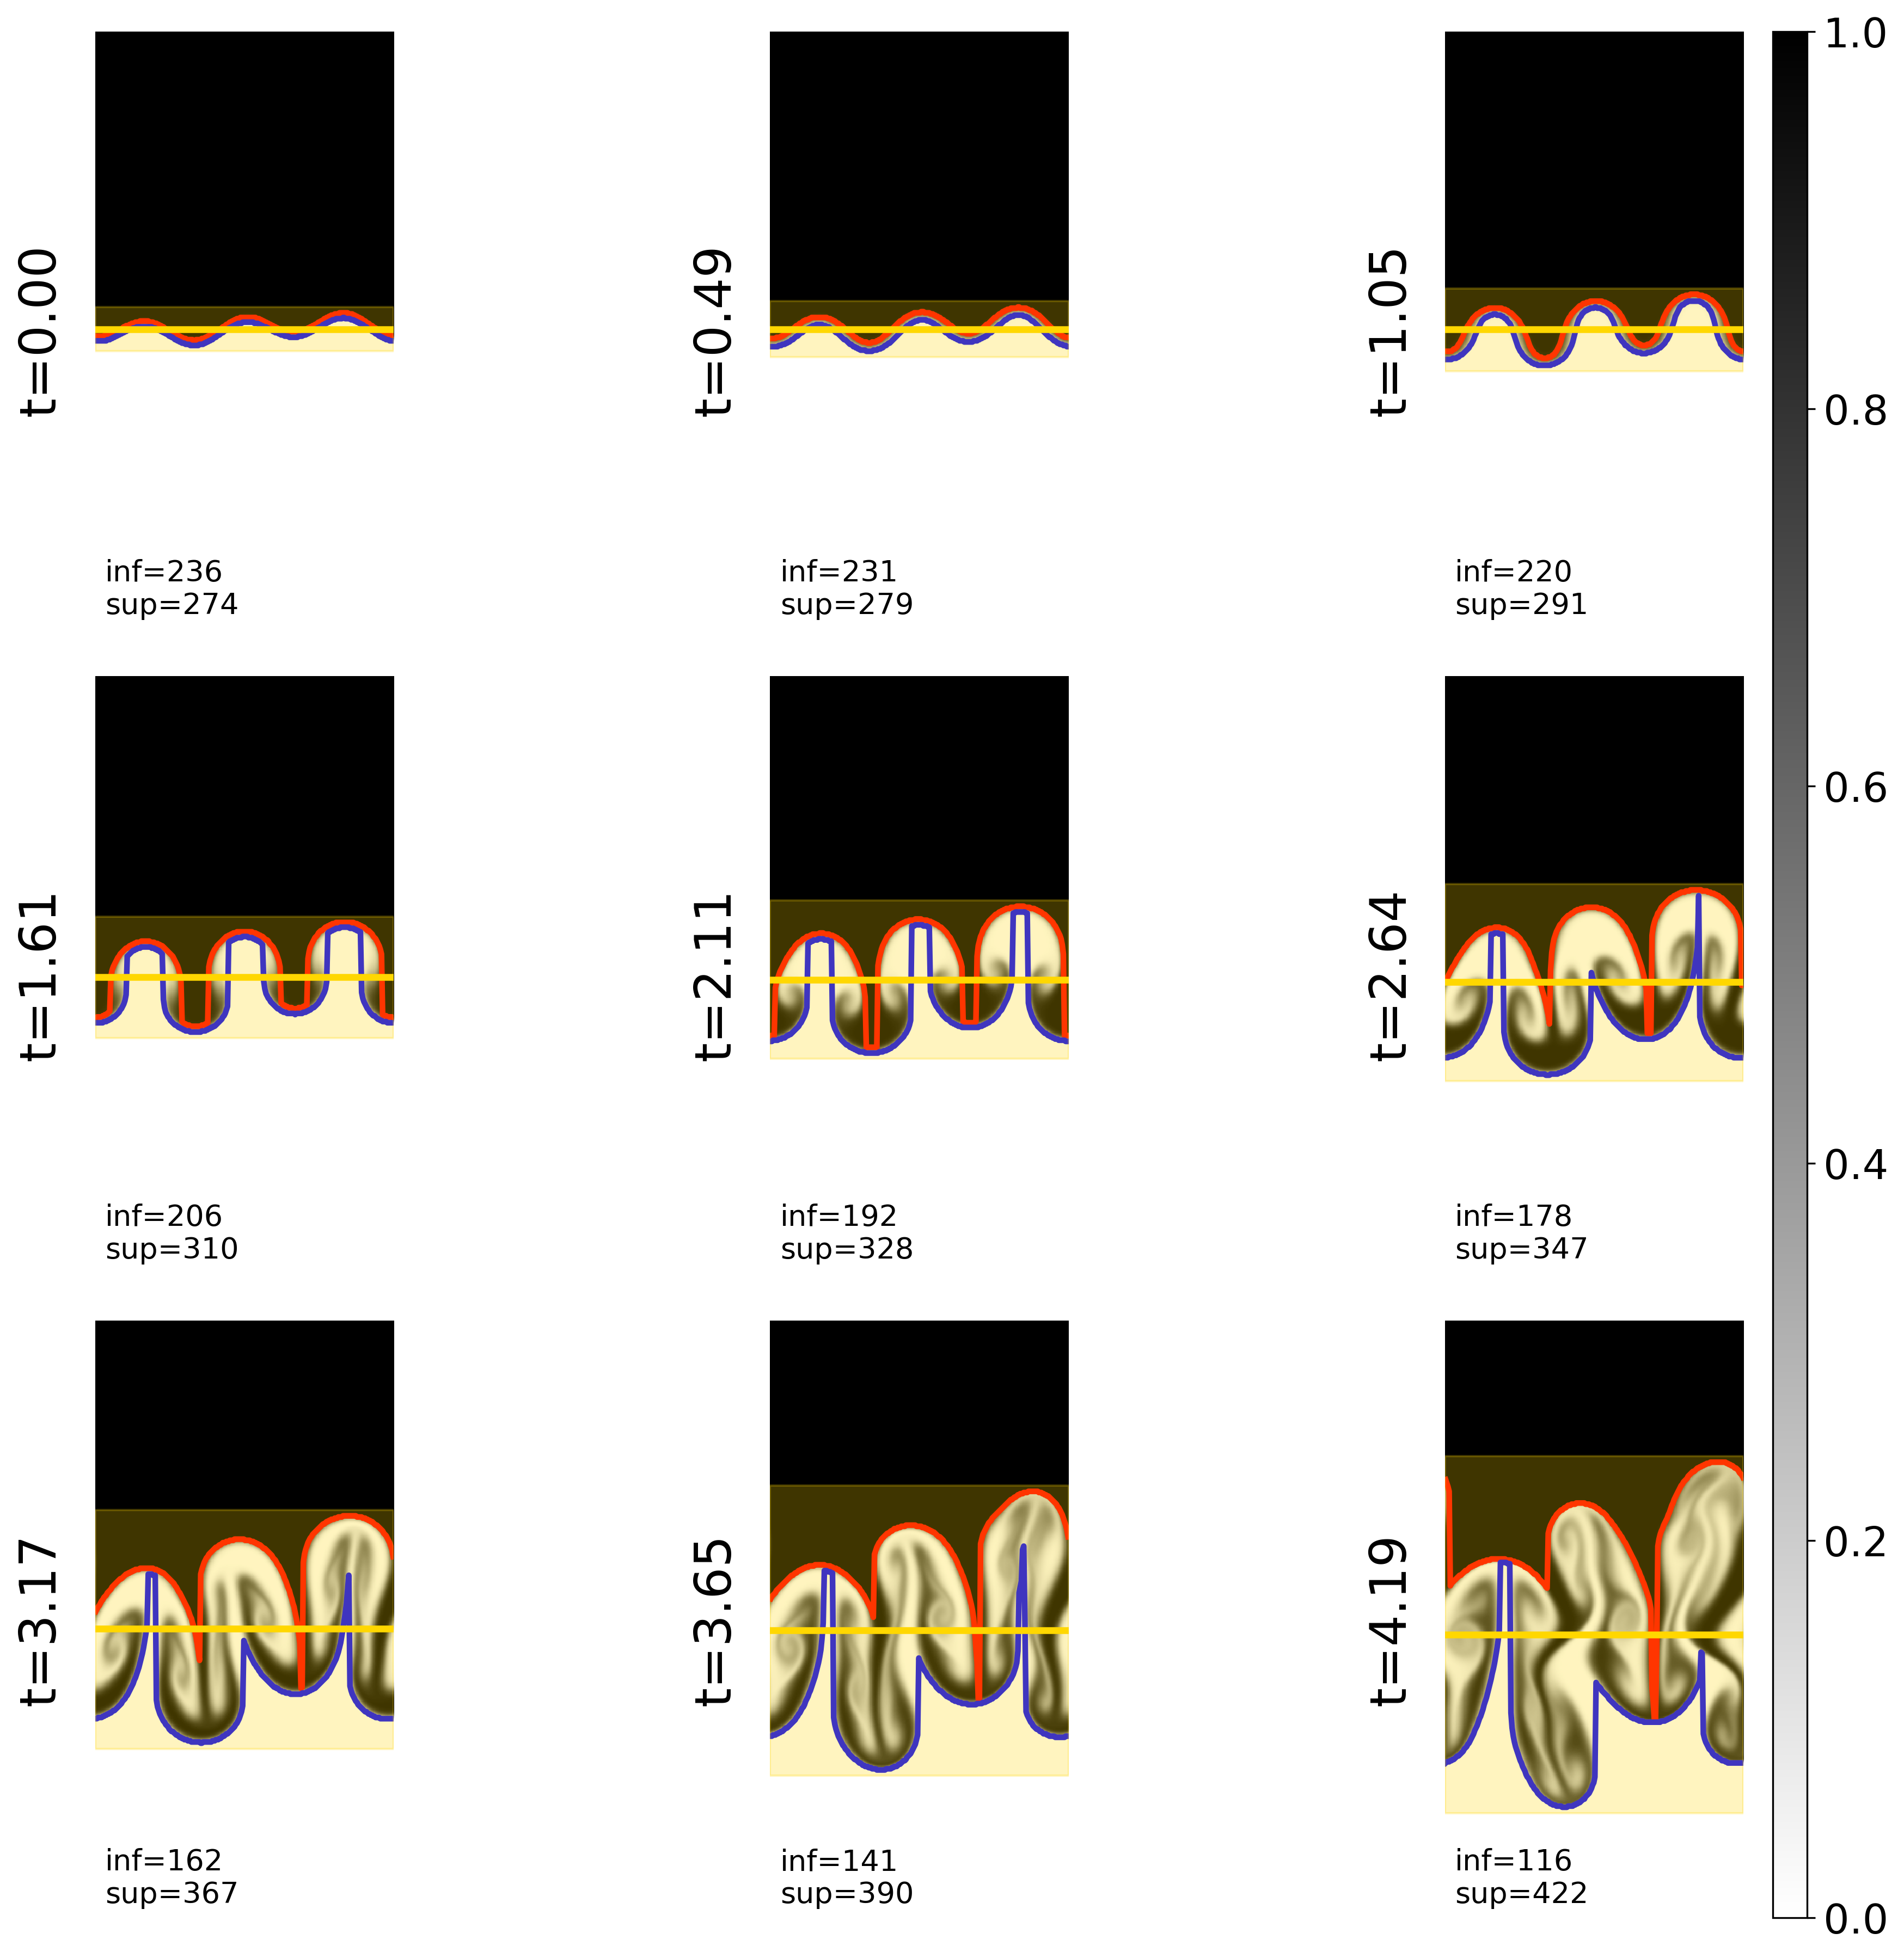
\includegraphics[width=0.65\textwidth]{figures/ch3/zone_melange.png}
\caption{Selection of the cropped field of view so that the whole mixing region remains inside the observation window.}
\label{fig:zone_melange}
\end{figure}

\subsection{Physically consistent data augmentation}

Because the data originate from numerical simulations, admissible
augmentations are constrained by the symmetries of the governing equations.
The pseudo-spectral solver uses periodic boundary conditions in the horizontal
direction, so cyclic horizontal translations preserve the physical content of
the samples. Horizontal reflection is also admissible because it corresponds to
the symmetry $x\rightarrow -x$.

The same is not true in the vertical direction. Vertical shifts modify the
position of the mixing layer relative to gravity, and vertical reflections
exchange light and heavy fluids while reversing the physical orientation of the
problem. Arbitrary rotations are excluded for the same reason. The
augmentation strategy is therefore deliberately restricted to horizontal
periodic shifts and horizontal flips.
The resulting admissible transformations are illustrated in
Figure~\ref{fig:augmentation}.

\begin{figure}[H]
    \centering
    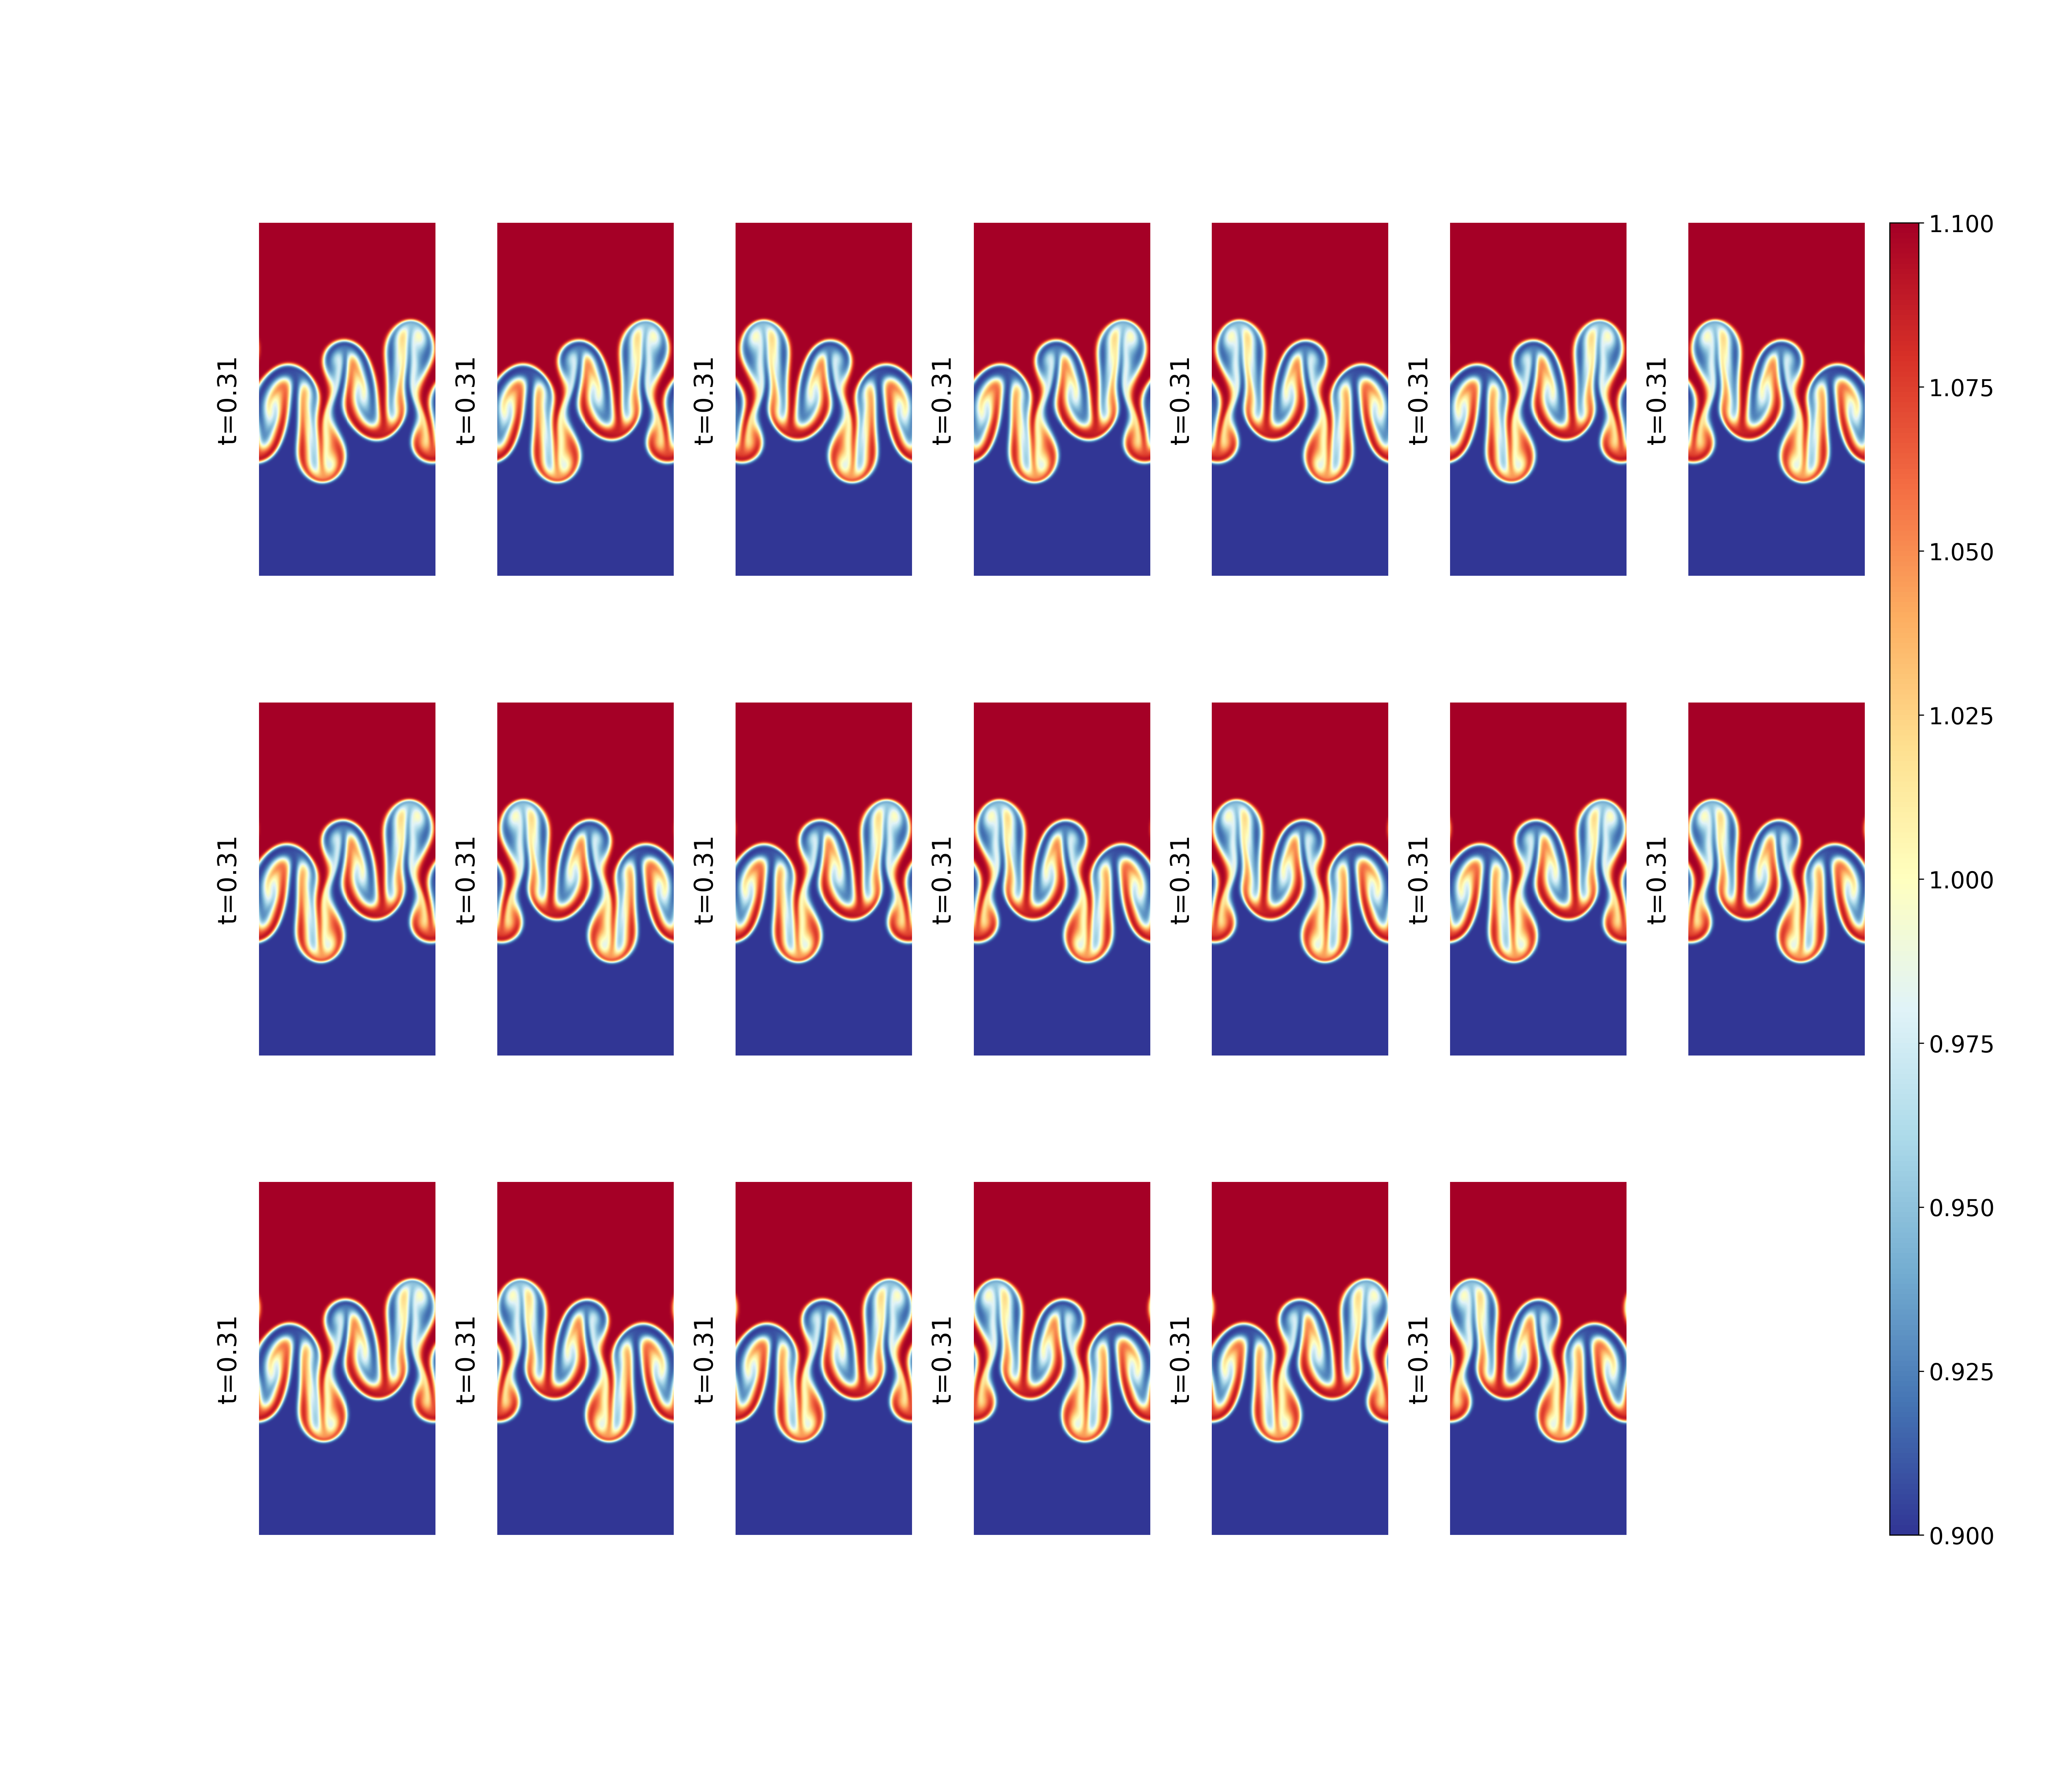
\includegraphics[width=0.95\textwidth]{figures/ch3/augmentation.png}
    \caption{Physically admissible augmentations for the RTI dataset: horizontal cyclic shifts and horizontal reflection only.}
    \label{fig:augmentation}
\end{figure}
